\chapter{Getting Started}

\section{System requirements}

Minsky is an open source program available for Windows, Mac OS X,
and various Linux distributions, as well as compilable on any suitable
Posix compliant system. Go to our \htmladdnormallink{SourceForge
page}{https://minsky.sourceforge.io} to download the version you need. Linux
packages are available from the \htmladdnormallink{OpenSUSE
build service}{https://build.opensuse.org/package/show/home:hpcoder1/minsky}.

\section{Getting help}

Press the F1 key, or select ``help'' from the context menu. Help is
context-sensitive.


\section{Components of the Program}

There are 6 components to the Minsky interface:

\begin{enumerate}
\item  The menus.

  \begin{tabular}{llllll}
    File & Edit & Insert & Options & Runge Kutta & Help \\
  \end{tabular}

\item  The Run buttons

\htmladdimg{NewItem15.png}

\item The simulation speed slider

\htmladdimg{NewItem16.png}

\item The Zoom buttons

\htmladdimg{NewItem17.png}

\item The Wiring and Equation tabs

\htmladdimg{WiringEquationsTab.png}

\item The design icons

\fwhtmladdimg{NewItem18.png}

\item And finally the Design Canvas--the large drawing area beneath the buttons and icons.

\fwhtmladdimg{NewItem19.png}
\end{enumerate}

\subsection{Menu}
\label{Menu}

  \begin{tabular}{llllll}
    File & Edit & Insert & Options & Runge Kutta & Help \\
  \end{tabular}

The menu controls the basic functions of saving and loading files,
default settings for the program, etc. These will alter as the program
is developed; the current menu items (as at the August 2016 Cantillon
release) are: 

\subsubsection{File}
\label{File}

\begin{description}
\item[About Minsky] Tells you the version of Minsky that you are using.

\item[New System] Clear the design canvas.

\item[Open] Open an existing Minsky file (Minsky files have the suffix of ``mky").

\item[Recent Files]\label{recentfiles} Provides a shortcut to some of
your previously opened Minsky files.

\item[Library] Opens a repository of models for the Minsky simulation system.

\item[Save] Save the current file.

\item[Save As] Save the current file under a new name.

\item[Insert File as Group] Insert a Minsky file directly into the
current model as a \htmlref{group}{Group}

\item[Export Canvas] Export the current canvas into *svg, *pdf, *eps, *tex, or *m format.
  If using LaTeX (*tex), produce the set of equations that define the
  current system for use in documenting the model, for use in LaTeX
  compatible typesetting systems. If your LaTeX implemention doesn't
  support breqn, untick the \htmlref{wrap long equations
  option}{wrap-equations}, which can be found in the preferences panel under the options menu.
  If using a MatLab function this can be used to simulate the system in a MatLab compatible system,
  such as \htmladdnormallinkfoot{MatLab}{https://en.wikipedia.org/wiki/MATLAB} or 
  \htmladdnormallinkfoot{Octave}{http://www.gnu.org/software/octave/}.

\item[Log simulation] Outputs the results of the integration variables
into a CSV data file for later use in spreadsheets or plotting
applications.

\item[Recording] Record the states of a model as it is being built for later
replay. This is useful for demonstrating how to build a model, but
bear in mind that recorded logs are not, in general, portable between
versions of Minsky.

\item[Replay recording] Replay a recording of model states.

\item[Quit] Exit the program. Minsky will check to see whether you have saved your changes. If you have, you will exit the program; if not, you will get a reminder to save your changes.

\item[Debugging use] Items under the line are intended for developer
  use, and will not be documented here. Redraw may be useful if the
  screen gets messed up because of a bug.

\end{description}

\subsubsection{Edit}
\label{Edit}

\begin{itemize}
\item\label{edit:undo} Undo and Redo allow you to step back and forward in your editing
history. If you step back a few steps, and then edit the model, all
subsequent model states will be erased from the history.

\item\label{edit:copy} Cut/copy/paste. Selecting, or lassoing a region
of the canvas will select a group of icons, which will be shaded to
indicate the selected items. Wires joining two selected items will
also be selected. Note that, compatible with X-windows, selecting
automatically performs a copy, so the copy operation is strictly
redundant, but provided for users familiar with systems where an
explicit copy request is required. Cut deletes the selected
items. Paste will paste the items in the clipboard as a
\htmlref{group}{Group} into the current model. At the time of writing,
copy-pasting between different instances of Minsky, or into other
applications, may not work on certain systems. Pasting the clipboard
into a text-based application will be a Minsky schema XML document.

%begin{latexonly}
\begin{tabular}{ccc}
\resizebox{0.45\textwidth}{!}{\includegraphics{images/selectionExamplePrior.eps}} & 
\raisebox{1.5cm}{$\Rightarrow$} &
\resizebox{0.45\textwidth}{!}{\includegraphics{images/selectionExamplePost.eps}}\\
\end{tabular}
%end{latexonly}
\begin{rawhtml}
<table>
<tr>
<td><img src="selectionExamplePrior.png"></td>
<td><big>&#x21d2;</big></td>
<td><img src="selectionExamplePost.png"></td>
</tr>
</table>
\end{rawhtml}

\item\label{edit:group} Create a \htmlref{group}{Group} using the
contents of the selection. Groups allow you to organise more
complicated systems specification into higher level modules that make
the overall system more comprehensible.

\end{itemize}

\subsubsection{Insert}
\label{Insert}

This menu contains a set of \htmlref{mathematical operator
blocks}{operations} for placement on the Canvas. You can get the same
effect by clicking on the Design Icons. Also present are entries for
\htmlref{Godley table items}{godley} and \htmlref{Plots}{PlotWidget}.


\subsubsection{Options}
\label{Options}

The options menu allows you to customise aspects of Minsky.

\begin{description}
\item[Preferences]\mbox{}

\begin{itemize}
\item Godley table show values. When ticked, the values of flow
variables are displayed in the Godley table whilst a simulation is
running. This will tend to slow down the simulation somewhat.
\item Godley table output style --- whether $+/-$ or DR/CR (debit/credit)
indicators are used.
\item Number of recent files to display --- affects the \htmlref{recent
files}{recentfiles} menu.
\item\label{wrap-equations} Wrap long equations in LaTeX export. If ticked, use the breqn
package to produce nicer looking automatically line-wrapped
formulae. Because not all LaTeX implementations are guaranteed to
support breqn, untick this option if you find difficulty.
\item\index{Panopticon} enable/disable the \htmlref{panopticon}{Panopticon}.
\end{itemize}

\item[Background colour] --- select a colour from which a colour scheme
is computed.

\end{description}

\subsubsection{Runge Kutta}
\label{RungeKutta}

\begin{itemize}
\item Controls aspect of the adaptive Runge-Kutta equation solver, which
trade off performance and accuracy of the model. 
\item Note a first order explicit solver is the classic Jacobi method, which is the fastest,
but least accurate solver. 
\item The algorithm is adaptive, so the
step size will vary according to how stiff the system of equations
is. 
\item Specifying a minimum step size prevents the system from stalling,
at the expense of accuracy when the step size reaches that
minimum. 
\item Specifying a maximum step size is useful to ensure one has
sufficient data points for smooth plots.
\item An iteration is the time between updates to plots, increasing the
number of solver steps per iteration decreases the overhead involved
in updating the display, at the expense of smoothness of the
plots. Screen refresh is the period between screen updates, in ms. If
an iteration takes less than this time, the screen refresh is postponed
until the time has expired. 100ms is fast enough for a smooth
animation of the simulation - increasing this value will improve
simulation performance at the cost of a jerky animation of the
simulation.
\item Start time is the value of the system $t$ variable when the
  system is reset.
\item Run until time can be used to pause the simulation ince t
  reaches a certain value. Setting this to ``Inf'' causes the
  simulation to run indefinitely, or until some arithmetic error
  occurs.
\end{itemize}

\subsubsection{Help}
\label{Help}

Provides an in-program link to this manual.

\subsection{Record/Replay Buttons}
\label{RecReplayButtons}

\htmladdimg{recReplayButtons.png}

These buttons control the recording / replay mode of Minsky. You can
record your interactions with Minsky, and replay those interactions
for demonstration/presentation purposes. 

\begin{enumerate}
  \item Record a session of building/modifying a model. Note that
    replaying a recorded session always starts from a blank canvas, so
    if you're recording the modification of a model, ensure that the
    first thing recorded is to load the model being modified. This
    button is a toggle button, so clicking it again finishes the
    session, and closes the file.
  \item Simulate/Replay button. Pressing this button changes Minsky
    into replay mode, and asks for a recording file. You may use the
    run buttons (run/pause,stop and step), as well as the speed
    slider, to control the replay. This button is a toggle button, so
    clicking it again returns Minsky back to the default simulation
    mode.
\end{enumerate}

\subsection{Run Buttons}
\label{RunButtons}

\htmladdimg{NewItem15.png}

The Run buttons respectively:
\begin{enumerate}
\item    Start a simulation--when started the button changes to a pause icon,
allowing you to pause the simulation \htmladdimg{NewItem23.png}.
\item Stop a simulation and reset the simulation time to zero
\item Step through the simulation one iteration at a time.
\end{enumerate}

%\subsection{Manipulating items on the canvas}
%
%\begin{description}
%\item[To move] and item, click on the interior of an item and drag it
%to the new position.
%\item[To wire items] click on the small circle representing the output
%port, and drag out a wire towards an input port on another item.
%\item[To lasso], click outside of any item and drag out a rectangular
%region.
%\item[To pan] the canvas, hold the shift key down whilst dragging on
%the canvas.
%\end{description}

%\begin{description}
%\item[Wire] This draws wires that connect one operator on the Canvas
%to another. For example, if you have placed these icons on the
%Palette: 
%
%\htmladdimg{NewItem24.png}
%
%and you now want to link them together into an equation, then click on
%the Wire button, move the cursor to the right end of GDP, and click
%and drag to the top of the divide symbol:
%
%\htmladdimg{NewItem25.png}
%
%Do the same for LabProd, and to attach the Divide icon to the left
%hand side of Workers, and you've defined the equation that the number
%of workers employed equals GDP divided by labor productivity. The
%flowchart will look like this: 
%
%\htmladdimg{NewItem26.png}
%
%And this is the equation you have now created:
%\begin{displaymath}
%\mathrm{Workers}=\frac{\mathrm{GDP}}{\mathrm{LabProd}}
%\end{displaymath}
%
%\item[Move] This is the default mode for the mouse, and it lets you:
%
%\begin{itemize}
%\item Move already entered icons around the Canvas by clicking on
%them, holding the mouse button down, and releasing it when you have
%got to the desired location; 
%\item Select an item from the Design Icons and place it on the
%Canvas. When you first click on an Icon, it will either appear at the
%top left hand corner of the Canvas, or bring up a menu where you enter
%various essential details (Name, value etc.), after which the Icon
%appears at the top left hand corner of the Canvas. It will then snap
%to wherever the mouse cursor currently is, and can be placed on the
%Canvas by clicking.
%\end{itemize}
%\item[Pan] This moves all the Icons on the Canvas as a group, which is useful
%when you have a very large model and you want to move to a small part
%of it. Choose Pan, click and hold the mouse button down, and then move
%the mouse. The entire model will shift with the mouse.
%
%\item[Lasso] Lassoing is the first step in creating a Group, or
%selecting multiple Icons for some operation (copying, deleting,
%etc.---these are not yet implemented but will be in the next major
%release).
%\end{description}
%
%        Grouping. Choose Lasso, click and hold down the mouse button,
%        then drag over the region you wish to make into a group:
%
%\htmladdimg{NewItem117.png}
%
%
%Release the mouse button, and a box will be drawn around the selected
%items which can now be moved as a single entity. The inputs to the
%group are noted on the input side of the group, and the outputs on the
%output side:
%
%\htmladdimg{NewItem118.png}
%
%One unique feature of Minsky (when compared to existing system
%dynamics programs) is that the contents of the group can still be seen
%inside the group window, and they can also be edited from there. In
%the next image, the contents of the group were moved more cleanly
%inside the group (this feature is still being implemented, so some
%tidying up was needed, but was possible without having to open the
%group in a separate window):
%
%
%\htmladdimg{NewItem119.png}

\subsection{Speed slider}
\label{Speedslider}

\begin{center}
\htmladdimg{NewItem16.png}
\end{center}

The speed slider controls the rate at which a model is simulated. The
default speed is the maximum speed your system can support, but you
can slow this down to more closely observe dynamics at crucial points
in a simulation.

\subsection{Zoom buttons}
\label{ZoomButtons}

\begin{center}
\htmladdimg{NewItem17.png}
\end{center}

The Zoom buttons zoom in and out on the wiring canvas. The same functionality
is accessed via the mouse scroll wheel. The reset zoom button
\buttonIcon{zoomOrig.eps} resets the zoom level to 1, and also
recentres the canvas. It can also be used to recentre the equation view.

\subsection{Simulation time}
\label{SimTime}

In the right hand top corner is a textual display of the current
simulation time $t$, and the current (adaptive) difference between
iterations $\Delta t$.

\subsection{Wiring and Equations Tabs}
\label{WiringEquationsTab}

\htmladdimg{WiringEquationsTab.png}

This allows you to switch between the visual block diagram wiring view and the more 
mathematical equations view.

\subsection{Design Icons}

\fwhtmladdimg{NewItem18.png}

These are the ``nuts and bolts'' of any system dynamics program. The
number of icons will grow over time, but the key ones are implemented
now: 

\begin{description}
\item[Godley Table] \buttonIcon{NewItem29.eps}. \label{GodleyTable} This is the
fundamental element of Minsky that is not found (yet) in any other
system dynamics program. 

Clicking on it and placing the resulting Bank Icon on the Canvas
enters a Godley table into your model:

\begin{center}

\includegraphics{images/NewItem29.eps}
\end{center}

Double-click on the Bank Icon (or right-click and choose ``Open Godley
Table'' from the context menu) and you get a double-entry bookkeeping
table we call a Godley Table, which looks like the following onscreen:

%\fwhtmladdimg{NewItem30.png}
\begin{center}
  \scalebox{0.5}{\includegraphics{images/emptyGodley.eps}}
\end{center}

 
Use this table to enter the bank accounts and financial flows in your model. We discuss this later in the \htmlref{Tutorial (Monetary)}{tut:basicBankModel}.

\item[Variable]  \buttonIcon{var.eps}. \label{Variable} This creates an entity
whose value changes as a function of time and its relationship with
other entities in your model. Click on it and a variable definition
window will appear:

\begin{center}
\scalebox{0.5}{\htmladdimg{NewItem32.png}}
\end{center}

The only essential step here is providing a name for the Variable. You
can also enter a value for it (and a rotation in degrees), but these
can be omitted. In a dynamic model, the value will be generated by the
model itself, provided its input is wired.


When you click on OK (or press Enter), the newly named variable will
appear in the top left hand corner of the Canvas. Move the mouse
cursor to where you want to place the variable on the Canvas, click,
and it will be placed in that location.


\item[Constant] \buttonIcon{const.eps} \label{Constant} creates an entity whose
value is unaffected by the simulation or other entities in the
model. Click on it and a constant definition window will appear:

\begin{center}
\scalebox{0.5}{\htmladdimg{NewItem34.png}}
\end{center}

The only essential element here is its
value. You can also specify its rotation on the Canvas in degrees. This lets you vary a
parameter while a simulation is running---which is useful if you wish
to explore a range of policy options while a model is running.

A constant is just a type of variable, which also include parameters
(named constants), flow variables, stock variables and integration
variables. In fact there is no real conceptual difference between
creating a constant or creating a variable, as you can switch the type
using the type field.

\item[Parameter] \buttonIcon{param.eps} \label{Parameter} Like the
  variable and constant button, this creates a variable defaulting to
  the parameter type. Parameters differ from flow variables in not
  having an input port, and differ from constants in having a name and
  being controllable by a slider during simulation.

\item[Time] \buttonIcon{time.eps} embeds a reference to the
simulation time on the Canvas. This is not necessary in most
simulations, but can be useful if you want to make a time-dependent
process explicit, or control the appearance of a graph. 

For example, by default a graph displays the simulation time on the
horizontal axis, so that cycles get compressed as a simulation runs
for a substantial period:

\begin{center}
\resizebox{\textwidth}{!}{\includegraphics{images/NewItem36.eps}}
\end{center}

If a Time block is added to the marker for the x-axis range, you can
control the number of years that are displayed. This graph is set up
to show a ten year range of the model only: 

\begin{center}
\resizebox{\textwidth}{!}{\includegraphics{images/NewItem37.eps}}
\end{center}



\item[Integration] \buttonIcon{int.eps}.\label{Integrate}
  This inserts a variable whose value depends on the integral of other
  variables in the system. This is the essential element for defining
  a dynamic model. Click on it and the following entity will appear at
  the top left hand side of the canvas (and move with your mouse until
  you click to place it somewhere:

\begin{center}

\includegraphics{images/NewItem39.eps}
\end{center}

``int1'' is just a placeholder for the integration variable, and the
first thing you should do after creating one is give it a
name. Double-click on the ``int1'', or right click and choose
Edit. This will bring up the following menu:

\begin{center}
\scalebox{0.5}{\htmladdimg{NewItem40.png}}
\end{center}

Change the name to something appropriate, and give it an initial
value. For example, if you were building a model that included
America's population, you would enter the following:

\begin{center}
\scalebox{0.5}{\htmladdimg{NewItem41.png}}
\end{center}


The integrated variable block would now look like this:

\begin{center}
\includegraphics{images/NewItem42.eps}
\end{center}


To model population, you need to include a growth rate. According to
Wikipedia, the current US population growth rate is 0.97 percent per
annum.  Expressed as an equation, this says that the annual change in
population, divided by its current level, equals 0.0097: 

\begin{displaymath}
\frac{1}{\mathrm{Population}(t)}\cdot\left(\frac{d}{dt}\mathrm{Population}(t)\right)=0.0097
\end{displaymath}

To express this as an integral equation, firstly we multiply both
sides of this equation by Population to get:

\begin{displaymath}
\frac{d}{dt}\mathrm{Population}(t)=0.0097\cdot\mathrm{Population}(t)
\end{displaymath}

Then we integrate both sides to get an equation that estimates what
the population will be T years into the future as:

\begin{displaymath}
\mathrm{Population}(T)=315+\int_0^T 0.0097\cdot\mathrm{Population}(t)
dt
\end{displaymath}

Here, 315 (million) equals the current population of the USA, the year
zero is today, and $T$ is some number of years from today. The same
equation done as a block diagram looks like this: 

\begin{center}
\resizebox{\textwidth}{!}{\includegraphics{images/NewItem46.eps}}
\end{center}

Or you can make it look more like the mathematical equation by
right-clicking on ``Population'' and choosing ``Copy Var''. Then you will
get another copy of the Population variable, and you can wire up the
equation this way:

\begin{center}
\resizebox{\textwidth}{!}{\includegraphics{images/NewItem47.eps}}
\end{center}

Either method can be used. I prefer the latter because it's neater,
and it emphasizes the link between the simple formula for a percentage
rate of change and a differential equation. 

\item[Derivative Operator] \buttonIcon{differentiate.eps} This operator symbolically differentiates its input,
provided the input is differentiable. An error is generated if the input
is not differentiable.

\item[Plus, Minus, Multiply and Divide blocks]
    \buttonIcon{add.eps}\buttonIcon{subtract.eps}\buttonIcon{multiply.eps}\buttonIcon{divide.eps}. These execute the stated binary
    mathematical operations. Each input can take multiple wires as
    well---so that to add five numbers together, for example you can wire 1 input
    to one port on the Add block, and the other four to the other
    port. 

\item[Min \& Max Functions] These take the minimum and maximum values, respectively.
These also allow multiple wires per input.

\item[Power and Logarithm] \buttonIcon{pow.eps} and
\buttonIcon{log.eps} These are binary operations (taking two
arguments). In the case of the power operation, the exponent is the
top port, and the argument to be raised to that exponent is the bottom
port. This is indicated by the $x$ and $y$ labels on the ports. In the
case of logarithm, the bottom port (labelled $b$) is the base of the
logarithm.

\item[Logical Operators $<$ $\le$, =, $\wedge$ $\vee$ $\neg$ (and,
  or, not)] \buttonIcon{lt.eps}, \buttonIcon{le.eps},
  \buttonIcon{eq.eps}, \buttonIcon{and_.eps}, \buttonIcon{or_.eps} and
  \buttonIcon{not_.eps}. These return 0 for false and 1 for true.

\item[Other functions] These are a fairly standard
complement of mathematical functions.

\item[Data block] \buttonIcon{data.eps} \htmlref{A data
block}{Operation:data} interpolates a sequence of empirical values, which may
be generated outside of Minsky, and imported as a CSV file. This
effectively defines a piecewise linear function.

\item[Plot widget] \buttonIcon{plot.eps} Add \htmlref{plots}{PlotWidget} to the canvas.

\item[Switch] \buttonIcon{switchIcon.eps} Add \htmlref{a piecewise-defined function block}{SwitchIcon} 
to the canvas. Also known as a hybrid function.

\item[Notes] Add \htmlref{textual annotations}{Notes}

\end{description}

\subsection{Design Canvas}
\label{DesignCanvas}

The Design Canvas is where you develop your model. A model consists of
a number of blocks---variables, constants and mathematical
operators---connected by wires. 

\fwhtmladdimg{NewItem19.png}

\subsection{The Panopticon}\label{Panopticon}

On the top right hand corner of the design canvas is a small recessed
panel showing a miniature version of the entire model, with the
current view port shown. This feature aids navigation around more
complex models. This feature may optionally be disabled through the
preferences panel, as it may cause unacceptable overheads for bigger models.

\subsection{Wires}
\label{Wires}

The wires in a model connect blocks together to define equations. For
example, to write an equation for 100/33, you would place a
\buttonIcon{const.eps} on the canvas, and give it the value of 100:

\begin{center}
\scalebox{0.5}{\htmladdimg{NewItem122.png}}
\end{center}

Then do the same for 33, and place a divide block on the canvas:

\begin{center}
\includegraphics{images/NewItem123.eps}
\end{center}

Then click on the right hand edge of \buttonIcon{const100.eps}
and drag to extend the wire to the numerator ($\times$) port of the divide operation.

\begin{center}
\includegraphics{images/wireExample1.eps}
\end{center}

Finally, add the other wire.
\begin{center}
\includegraphics{images/wireExample2.eps}
\end{center}

\section{Working with Minsky}

\subsection{Components in Minsky}

There are a number of types of components in Minsky
\begin{enumerate}
\item Mathematical operators such as plus (+), minus (-)
\item Constants (or parameters, which are named constants) which are
given a value by the user 
\item Variables whose values are calculated by the program during a simulation and depend on the values of constants and other variables; and
\item Godley Tables, which define both financial accounts and the
flows between them. In the language of stock and flow modelling, the
columns of a Godley table are the stocks, which are computed by
integrating over a linear combination of flow variables.
\item Integrals --- represent a variable computed by integrating a
function forward in time.
\item Groups, which allow components to be grouped into modules that
can be used to construct more complex models.
\end{enumerate}


\subsection{Inserting a model component}


There are three ways to insert a component of a model onto the Canvas:
\begin{enumerate}
\item Click on the desired Icon on the Icon Palette, drag the block
onto the Canvas and release the mouse where you want to insert it 

\begin{center}
\fwhtmladdimg{NewItem18.png}
\end{center}

\item Choose Insert from the menu and select the desired block there

  \begin{center}
    %begin{latexonly}
    \resizebox{!}{0.6\textheight}{
      %end{latexonly}
      \htmladdimg{NewItem159.png}
     %begin{latexonly}
    }
    %end{latexonly}
  \end{center}
  \newpage
  
\item Right-click on an existing block and choose copy. Then place the
copy where you want it on the palette. 

\begin{center}
\htmladdimg{NewItem161.png}
\end{center}


\end{enumerate}

\subsection{Creating an equation}

Equations are entered in Minsky graphically. Mathematical operations
like addition, multiplication and subtraction are performed by wiring
the inputs up to the relevant mathematical block. The output of the
block is then the result of the equation. 

For example, a simple equation like
\begin{displaymath}
100/3 = 33.3
\end{displaymath}
is performed in Minsky by defining a constant block with a value of 100, defining another with a value of 3, and wiring them up to a divide-by block. Then attach the output of the divide block to a variable, and run the model by clicking on\smhtmladdimg{NewItem130.png} :

\begin{center}
  \includegraphics{images/NewItem129.eps}
\end{center}

If you click on the equation tab, you will see that it is:

\begin{displaymath}
\mathrm{Answer}=\frac{100}{3}
\end{displaymath}

Very complex equations---including dynamic elements like integral
blocks and Godley Tables---are designed by wiring up lots of
components, with the output of one being the input of the next. See
the tutorial for examples.

\subsection{Wiring components together}

A model is constructed by wiring one component to another in a way
that defines an equation. Wires are drawn from the output port of one
block to the input port of another. Ports are circles on the blocks to
which wires can be attached, which can be seen when hovering the
pointer over the block. Variables have an input and an output
port; constants and parameters only have an output port. A
mathematical operator has as many input ports as are needed to define
the operation.


To construct an equation, such as Fred - Wilma = Barney:

Click the mouse near the output port of one block and drag the
cursor to the input port of another while holding the mouse button
down. An arrow extends out from the output port. Release the mouse
button near the required input port of the operator. A connection will
be made.

\begin{center}
\includegraphics{images/NewItem181.eps} 
\end{center}


The equation is completed by wiring up the other components in the same way.

\begin{center}
\includegraphics{images/NewItem182.eps} 
\end{center}


\subsection{Creating a banking model}
\label{creatingBankingModel}

\subsubsection{Creating a bank}

The first step in creating a model with a banking sector is to click on the Godley Table Icon in the Icon Palette, and place the block somewhere on the Canvas.

\subsubsection{Entering accounts}

Double click or right click on the Godley table block to bring up the
Godley Table. The table is divided up into sections representing the
different accounting asset classes: Asset, Liability and
Equity. Assets represent what you have to hand at any point in time,
and should always be the sum of liabilities and equity. Liabilities
represent amounts that are owed to other parties, and equity the
amount of capital owned. The column \verb+A-L-E+ represents the {\em
  accounting equation} (Assets$-$Liabilities$-$Equity), and a properly
formatted Godley table adhering to {\em double entry accounting
  conventions} will have this column zero for all rows.

When a Godley Table is first loaded, each accounting class has room
for one account (also known as a {\em stock}) to be defined. To create
an additional accounts, click on the `+' button above the first
account. One click then adds another column in which an additional
account can be defined. Note that the table will delete excess blank
accounts, so you should name them as you go. You can chancge the asset
class of an account by moving it into the appropriate sector using the
$\leftarrow$ and $\rightarrow$ buttons, or by clicking and dragging
the column variable name (the first row of the column).

%\begin{center}
%\begin{tabular}{|c|cc|}
%\hline
%Flows $\downarrow$ / Stock Variables $\rightarrow$&\multicolumn{1}{|c|}{}&\multicolumn{1}{|c|}{}\\\cline{2-3}&\multicolumn{2}{|c|}{noAssetClass}\\\hline
%Initial Conditions&$0$&$0$\\
%\hline
%\end{tabular}
%\end{center}

\begin{center}
  \scalebox{0.5}{\includegraphics{images/emptyGodley.eps}}
\end{center}


A column can be deleted by clicking on the `--' button above the column.

To define bank accounts in the system you enter a name into the row
labeled ``Flows $\downarrow$ / Stock Variables $\rightarrow$''. For example, if you were
going to define a banking sector that operated simply as an
intermediary between ``Patient'' people and ``Impatient'' people---as
in the Neoclassical ``Loanable Funds'' model--you might define the
following accounts: 

%\begin{center}
%\begin{tabular}{|c|cccc|}
%\hline
%Flows $\downarrow$ / Stock Variables $\rightarrow$&\multicolumn{1}{|c|}{$Reserves$}&\multicolumn{1}{|c|}{$Patient$}&\multicolumn{1}{|c|}{$Impatient$}&\multicolumn{1}{|c|}{$Safe$}\\\cline{2-5}&\multicolumn{4}{|c|}{noAssetClass}\\\hline
%Initial Conditions&$0$&$0$&$0$&$0$\\
%\hline
%\end{tabular}
%\end{center}

\begin{center}
  \scalebox{.5}{\includegraphics{images/godleyTableWithAccounts.eps}}
\end{center}


As you enter the accounts, they appear at the bottom of the Bank block on the canvas:

\begin{center}
  \scalebox{0.5}{\includegraphics{images/NewItem145.eps}}
\end{center}

%\subsection{Defining account types}
%
%Bank accounts must be classified as either an Asset, a Liability, or
%the Equity of the relevant Bank, using the drop-down menu currently
%labeled {\tt noAssetClass} at the top of each account. In
%this model, Reserves are an asset of the banking sector, the accounts
%of ``Patient'' and ``Impatient'' are liabilities, and the ``Safe'' is
%the equity of the banking system. Click on the
%{\tt noAssetClass} button and this drop-down menu will
%appear:
%
%\begin{center}
%\htmladdimg{NewItem140.png} 
%\end{center}
%
%Choose the relevant entry for each column, and the accounts will be properly classified when the model is simulated:
%
%\begin{center}
%\begin{tabular}{|c|cccc|}
%\hline
%Flows $\downarrow$ / Stock Variables $\rightarrow$&\multicolumn{1}{|c|}{$Reserves$}&\multicolumn{1}{|c|}{$Patient$}&\multicolumn{1}{|c|}{$Impatient$}&\multicolumn{1}{|c|}{$Safe$}\\\cline{2-5}&\multicolumn{1}{|c|}{asset}&\multicolumn{2}{|c|}{liability}&\multicolumn{1}{|c|}{equity}\\\hline
%Initial Conditions&$0$&$0$&$0$&$0$\\
%\hline
%\end{tabular}
%\end{center}

\subsubsection{Entering flows between accounts}


Flows between accounts are entered by typing text labels in the
accounts involved. The source label is entered as a simple name---for
example, if Patient is lending money to Impatient, the word ``Lend''
could be used to describe this action. Firstly you need to create a
row beneath the ``Initial Conditions'' row (which records the amount of
money in each account when the simulation begins). You do this by
clicking on the `+' key on the Initial Conditions row. This creates a
blank row for recording a flow between accounts.

%\begin{center}
%\begin{tabular}{|c|cccc|}
%\hline
%Flows $\downarrow$ / Stock Variables $\rightarrow$&\multicolumn{1}{|c|}{$Reserves$}&\multicolumn{1}{|c|}{$Patient$}&\multicolumn{1}{|c|}{$Impatient$}&\multicolumn{1}{|c|}{$Safe$}\\\cline{2-5}&\multicolumn{1}{|c|}{asset}&\multicolumn{2}{|c|}{liability}&\multicolumn{1}{|c|}{equity}\\\hline
%Initial Conditions&$0$&$0$&$0$&$0$\\
%&&&&\\
%\hline
%\end{tabular}
%\end{center}

\begin{center}
  \scalebox{.5}{\includegraphics{images/godleyTableWithAccounts1.eps}}
\end{center}

The cell below ``Initial Conditions'' is used to give a verbal
description of what the flow is: 

%\begin{center}
%\begin{tabular}{|c|cccc|}
%\hline
%Flows $\downarrow$ / Stock Variables $\rightarrow$&\multicolumn{1}{|c|}{$Reserves$}&\multicolumn{1}{|c|}{$Patient$}&\multicolumn{1}{|c|}{$Impatient$}&\multicolumn{1}{|c|}{$Safe$}\\\cline{2-5}&\multicolumn{1}{|c|}{asset}&\multicolumn{2}{|c|}{liability}&\multicolumn{1}{|c|}{equity}\\\hline
%Initial Conditions&$0$&$0$&$0$&$0$\\
%Patient lends to Impatient&&&&\\
%\hline
%\end{tabular}
%\end{center}
\begin{center}
  \scalebox{.5}{\includegraphics{images/godleyTableWithAccounts2.eps}}
\end{center}

The flows between accounts are then recorded in the relevant cells
underneath the columns. Here we will start with putting the label
``-Lend'' into the Patient column. It is negative, because Patient is
lending to Impatient.

%\begin{center}
%\begin{tabular}{|c|cccc|}
%\hline
%Flows $\downarrow$ / Stock Variables $\rightarrow$&\multicolumn{1}{|c|}{$Reserves$}&\multicolumn{1}{|c|}{$Patient$}&\multicolumn{1}{|c|}{$Impatient$}&\multicolumn{1}{|c|}{$Safe$}\\\cline{2-5}&\multicolumn{1}{|c|}{asset}&\multicolumn{2}{|c|}{liability}&\multicolumn{1}{|c|}{equity}\\\hline
%Initial Conditions&$0$&$0$&$0$&$0$\\
%Patient lends to Impatient&&$-Lend$&&\\
%\hline
%\end{tabular}
%\end{center}
\begin{center}
  \scalebox{.5}{\includegraphics{images/godleyTableWithAccounts3.eps}}
\end{center}

Notice that the program shows that the Row Sum for this transaction is
currently ``Lend'', when it should be zero to obey the double-entry
bookkeeping rule that all rows must balance. This is because a
destination for ``Lend'' has not yet been specified. Please note that different
asset class columns follow different +ve and -ve rules, so an asset and a liability
with the same value might need to both be +ve or both -ve to sum to zero. The destination
is Impatient's account, and to balance the row to zero this part of
the transaction must be entered as ``Lend'': 

%\begin{center}
%\begin{tabular}{|c|cccc|}
%\hline
%Flows $\downarrow$ / Stock Variables $\rightarrow$&\multicolumn{1}{|c|}{$Reserves$}&\multicolumn{1}{|c|}{$Patient$}&\multicolumn{1}{|c|}{$Impatient$}&\multicolumn{1}{|c|}{$Safe$}\\\cline{2-5}&\multicolumn{1}{|c|}{asset}&\multicolumn{2}{|c|}{liability}&\multicolumn{1}{|c|}{equity}\\\hline
%Initial Conditions&$0$&$0$&$0$&$0$\\
%Patient lends to Impatient&&$-Lend$&$Lend$&\\
%\hline
%\end{tabular}
%\end{center}
\begin{center}
  \scalebox{.5}{\includegraphics{images/godleyTableWithAccounts4.eps}}
\end{center}

The accounting equation also applies to the Initial Conditions (the amount of money
in each of the accounts prior to the flows between accounts): the
Initial Conditions must balance. This requires that there are
entries on the Asset side of the Banking ledger that exactly match the
sum of Liabilities and Equity: 

%\begin{center}
%\begin{tabular}{|c|cccc|}
%\hline
%Flows $\downarrow$ / Stock Variables $\rightarrow$&\multicolumn{1}{|c|}{$Reserves$}&\multicolumn{1}{|c|}{$Patient$}&\multicolumn{1}{|c|}{$Impatient$}&\multicolumn{1}{|c|}{$Safe$}\\\cline{2-5}&\multicolumn{1}{|c|}{asset}&\multicolumn{2}{|c|}{liability}&\multicolumn{1}{|c|}{equity}\\\hline
%Initial Conditions&$120$&$100$&$0$&$20$\\
%Patient lends to Impatient&&$-Lend$&$Lend$&\\
%\hline
%\end{tabular}
%\end{center}
\begin{center}
  \scalebox{.5}{\includegraphics{images/godleyTableWithAccounts5.eps}}
\end{center}

As you enter flows, these appear on the left hand side of the bank block:

\begin{center}
  \scalebox{0.5}{\includegraphics{images/NewItem147.eps}}
\end{center}

\subsubsection{Defining flows}

The entries in the Godley Table represent flows of money, which are
denominated in money units per unit of time. The relevant time
dimension for an economic simulation is a year (whereas in engineering
applications, the relevant time dimension is a second), so whatever
you enter there represents a flow of money per year.


You define the value of flows by attaching a constant or variable to
the input side of the flow into the bank as shown on the Canvas. For
example, you could assign Lend a value of 10 (which would represent a
loan of \$10 per year by Patient to Impatient) by:



Create a constant with a value of 10, and attaching this to the input
side of Lend:

\begin{center}
\scalebox{0.5}{\includegraphics{images/NewItem149.eps}}
\end{center}

What you have now defined is an annual flow from Patient to Impatient
of \$10. In the dynamic equations this model generates, Minsky
converts all amounts in accounts to positive sums---it shows the
financial system from the point of the overall economy, rather than
from the point of view of the bank:

\begin{eqnarray*}
\mathrm{Lend}&=&10\\
\frac{d\mathrm{Impatient}}{dt}&=&\mathrm{Lend}\\
\frac{d\mathrm{Patient}}{dt}&=&-\mathrm{Lend}\\
\frac{d\mathrm{Reserves}}{dt}&=&\\
\frac{d\mathrm{Safe}}{dt}&=&
\end{eqnarray*}



If you attach a graph to the accounts at the bottom of the bank block,
you will see the impact of this flow over time on the balances of the
two accounts. Patient's account begins at \$100 and falls at \$10 per
year, while Impatient's account begins at \$0 and rises by \$10 per
year.

\begin{center}
\scalebox{0.7}{\includegraphics{images/NewItem151.eps}}
\end{center}

Obviously this will result in a negative total worth for Patient after
10 years, so it is not a realistic model. A more sensible simple model
would relate lending to the amount left in Patient's account (and a
more complex model would relate this to many other variables in the
model). That is done in the next example, where a constant ``lendrate''
has been defined and given the value of 0.1, and Lend is now defined
as 0.1 times the balance in Patient's account. This now results in a
smooth exponential decay of the amount in the Patient account, matched
by a rise in the amount in Impatient account.

\begin{center}
\scalebox{0.7}{\includegraphics{images/NewItem152.eps}}
\end{center}

This is because the equation you have defined is identical to a
radioactive decay equation, with the amount in the Patient account
falling at 10 percent per year:

\begin{eqnarray*}
\mathrm{Lend}&=&\mathrm{lendrate}\times\mathrm{Patient}\\
\frac{d\mathrm{Impatient}}{dt}&=&\mathrm{Lend}\\
\frac{d\mathrm{Patient}}{dt}&=&-\mathrm{Lend}\\
\end{eqnarray*}

Note however that there are now wires crossing over other wires? There
is a neater way to define flows. 

\subsubsection{Copying Godley Table input \& outputs}

Right-click on the inputs and outputs of a Godley Table and choose
``copy'' from the drop-down menu:

\begin{center}
\htmladdimg{NewItem153.png}
\end{center}

Place the copied flows and accounts and place them away from the
table. Then wire up your definition there:


\begin{center}
\includegraphics{images/NewItem154.eps}
\end{center}


This now results in a much neater model. The same process can be used
to tidy up graphs as well:

\begin{center}
\resizebox{\textwidth}{!}{\includegraphics{images/NewItem155.eps}}
\end{center}


A more complex model would have many more flows, and these in turn
would depend on other entities in the model, and be time-varying
rather than using a constant ``lendrate'' as in this example---see the
Tutorial on a \htmlref{Basic Banking Model}{tut:basicBankModel} for an
example. This example uses the engineering concept of a
\htmlref{``time constant''}{time-constants}, which is explained in the
next section. Please note that right-clicking godley table variables and
selecting "copy flow variables" creates a new group, which, when clicked and
selecting "open in canvas", changes the canvas to show just that group. The normal
canvas can be brought back by right-clicking and selecting "open master group".

\subsubsection{Using ``Time Constants''}
\label{time-constants}

The value of 0.1 means that the amount of money in the Patient account
falls by one tenth every year (and therefore tapers towards zero). An
equivalent way to express this is that the ``time constant'' for
lending is the inverse of 1/10, or ten years. The next model uses a
variable called $\tau_{Lend}$, and gives it a value of 10: 

\begin{center}
\includegraphics{images/NewItem158.eps}
\end{center}

As the simulation shows, the two models have precisely the same result
numerically:

\begin{center}
\resizebox{!}{0.9\textheight}{\includegraphics{images/NewItem157.eps}}
\end{center}


The advantage of the time constant approach is that it is defined in
terms of the time that a process takes. A time constant of 10 says
that, if this rate of lending was sustained (rather than declining as
the account falls), then in {\bf\em precisely} 10 years, the Patient account
would be empty. The advantages of this formulation will be more
obvious in the \htmlref{tutorial}{tutorial}.


\subsubsection{Multiple banks}

There can be any number of Godley Tables---each representing a
different financial institution or sector in an economy---in the one
diagram. The name of the institution can be altered by clicking on the
default name (``Godley0'' in the first one created) and altering
it. Here is an example with 4 such institutions/sectors defined:


\begin{center}
\includegraphics{images/NewItem136.eps}
\end{center}

If there are interlocking accounts in these banks---if one lends to
another for example---then what is an asset for one must be shown as a
liability for the other. 

Godley tables may be further placed in {\em groups}, which allows
scoping of the flow variables and their defining equations, whilst
still allowing the tables to be coupled via global variables.
